\documentclass[reprint,aps,pre,amsmath,amssymb,superscriptaddress,showpacs]{revtex4-1}
\usepackage{graphicx,float}

\begin{document}

\title{Erratum: Tropical approximation to finish time of activity networks [Phys. Rev. E 106, L012301 (2022)]}

\author{Alexei Vazquez}
\email{alexei@nodeslinks.com}
\affiliation{Nodes \& Links}

\maketitle
The figures for simulated projects have an error in the original paper. The code to calculate the free floats was using $w_{ij} = y_j - x_i$ instead of the correct expression $w_{ij} = x_j - x_i$ (see Eq. (3)). This error is the actual cause of the anomalies observed in the small $\sigma$ region in Figs. 2 and 3. After correcting this coding error,  the new Figs. 1, and 3 are shown here. The data for real project networks (Figs. 4 and 5) is not affected by this Erratum. Based on this evidence I conclude that the tropical approximation is valid for $\sigma\gg1$, where $\sigma$ is the variance of the logarithm of exogenous delays.

\begin{figure}[t]
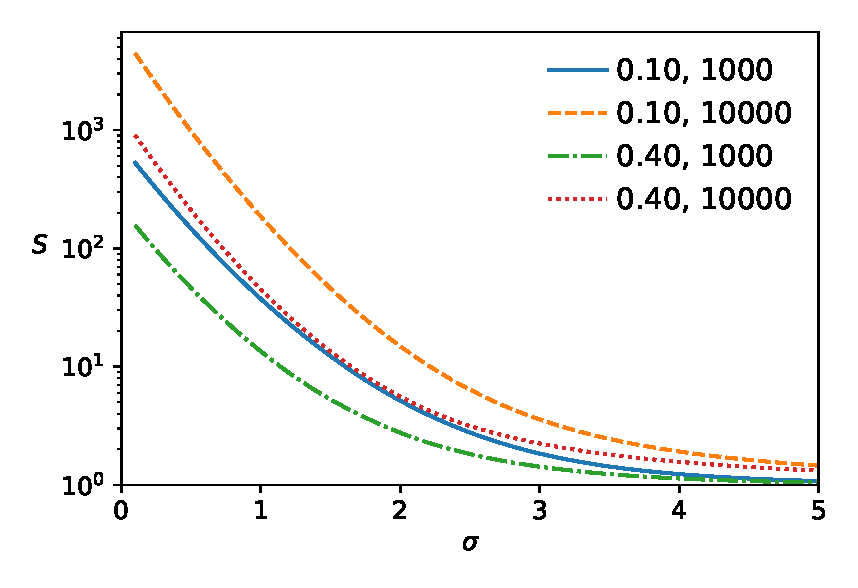
\includegraphics[width=3.3in]{maxsum.scheduling.dupsplit.arc_distribution_zero.eps}
\caption{Slope between the calculated p80s using $f={\rm sum}$ vs using $f={\max}$, for $\vec{d}=\vec{0}$ and the $(q,n)$ indicated in the legend.}
\label{fig1}
\end{figure}

\begin{figure}[b]
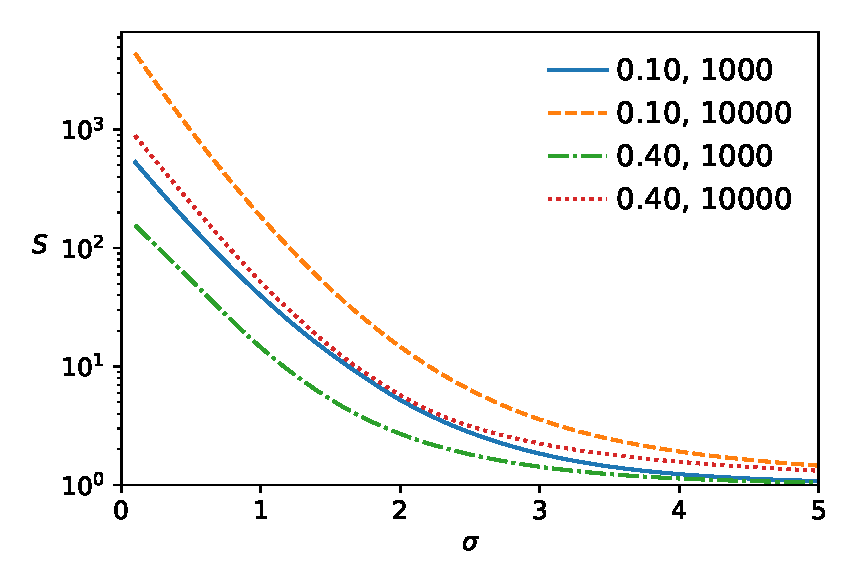
\includegraphics[width=3.3in]{maxsum.scheduling.dupsplit.arc_distribution_lognormal.arc_sigma_1.eps}
\caption{Slope between the calculated p80s using $f={\rm sum}$ vs using $f={\max}$, for $\sigma_1=1$ and the $(q,n)$ indicated in the legend. }
\label{fig2}
\end{figure}

\begin{figure}[t]
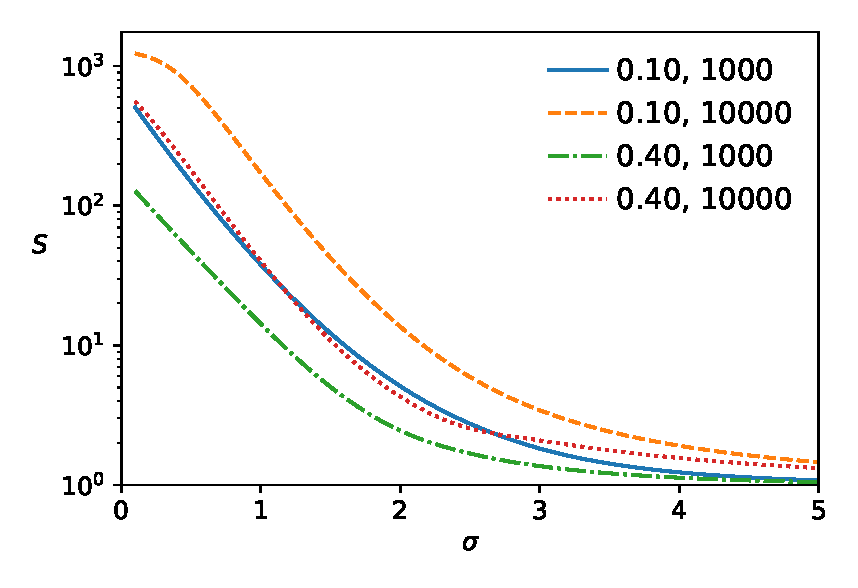
\includegraphics[width=3.3in]{maxsum.scheduling.dupsplit.arc_distribution_lognormal.arc_sigma_3.eps}
\caption{Slope between the calculated p80s using $f={\rm sum}$ vs using $f={\max}$, for $\sigma_1=3$ and the $(q,n)$ indicated in the legend. }
\label{fig3}
\end{figure}



\end{document}
